\documentclass{article}

% Language setting
% Replace `english' with e.g. `spanish' to change the document language
\usepackage[english]{babel}

% Set page size and margins
% Replace `letterpaper' with `a4paper' for UK/EU standard size
\usepackage[letterpaper,top=2cm,bottom=2cm,left=3cm,right=3cm,marginparwidth=1.75cm]{geometry}

% Useful packages
\usepackage{amsmath}
\usepackage{graphicx}
\usepackage[colorlinks=true, allcolors=blue]{hyperref}
\usepackage[dvipsnames]{xcolor}
\title{Your Paper}
\author{You}

\begin{document}
\maketitle

\begin{abstract}
Your abstract.
\end{abstract}

\section{Introduction}


\textcolor{Aquamarine} {For this presentation, I am going to mark-up the already excellent default example project in Overleaf. You can experiment with this stuff yourself in Overleaf by going to New Project from the main menu, selecting "Example Project" and replacing main.tex with this version of main.tex. Text in Aquamarine will be my comments, while text in black will be from the Overleaf example. First, a roadmap: \LaTeX{} is a code-based document editor as compared to more familiar interactive document editors such as Word. In Overleaf, there are three panels. The leftmost navigation panel shows you all of the components of the current project. In addition to the manuscript that we are working on (main.tex), we also have an image file and a bibliography. The middle panel is the code-editor. This is where you will write your manuscript. You can toggle back and forth between Code Editor and Visual Editor modes depending on which makes you more comfortable. The right panel shows you the final product. You will need to press the green Recompile button to update after any changes made in the code-editor. The Download button to the right of the recompile button will download the right panel into a PDF.}



Your introduction goes here! Simply start writing your document and use the Recompile button to view the updated PDF preview. Examples of commonly used commands and features are listed below, to help you get started.

Once you're familiar with the editor, you can find various project settings in the Overleaf menu, accessed via the button in the very top left of the editor. To view tutorials, user guides, and further documentation, please visit our \href{https://www.overleaf.com/learn}{help library}, or head to our plans page to \href{https://www.overleaf.com/user/subscription/plans}{choose your plan}.

\textcolor{Aquamarine}{Any unaccompanied text on a line is treated as text for the manuscript. Blank lines, such as the one above, are treated as paragraph breaks. If your project fails to recompile, or if something you have added to the code editor is missing in the PDF in the right column, it is likely that you have made an error in your code. Errors and warning will show up next to the line numbers in the right hand side of this panel. Mouse over them to gain more information. I'll include a non-fatal error in the next line as an example. }
\includegraphics[]{}

\textcolor{Aquamarine}{I have attempted to include an image, but have failed to specify which one. The Red dot tells me the file is not found, but because it doesn't affect the other lines (such as an unclosed bracket might), the rest of the document can still compile, and it just ignores the broken command. Some Commands are native to overleaf, while others are user-written, much like an R-package or Stata .ado file. To add user-created packages, simply add a usepackage command to the preamble of your code. If you look at the code for this paper, in addition to the example packages, I have included xcolor, which is what is allowing me to write in} \textcolor{Fuchsia}{different} \textcolor{BrickRed}{colors.}\textcolor{Aquamarine}{I have also added Tikz, which will allow us to make Graphs later.}

\section{Some examples to get started}

\subsection{How to create Sections and Subsections}

Simply use the section and subsection commands, as in this example document! With Overleaf, all the formatting and numbering is handled automatically according to the template you've chosen. If you're using the Visual Editor, you can also create new section and subsections via the buttons in the editor toolbar.

\subsection{How to include Figures}

First you have to upload the image file from your computer using the upload link in the file-tree menu. Then use the includegraphics command to include it in your document. Use the figure environment and the caption command to add a number and a caption to your figure. See the code for Figure \ref{fig:frog} in this section for an example.

Note that your figure will automatically be placed in the most appropriate place for it, given the surrounding text and taking into account other figures or tables that may be close by. You can find out more about adding images to your documents in this help article on \href{https://www.overleaf.com/learn/how-to/Including_images_on_Overleaf}{including images on Overleaf}.

\begin{figure}
\centering
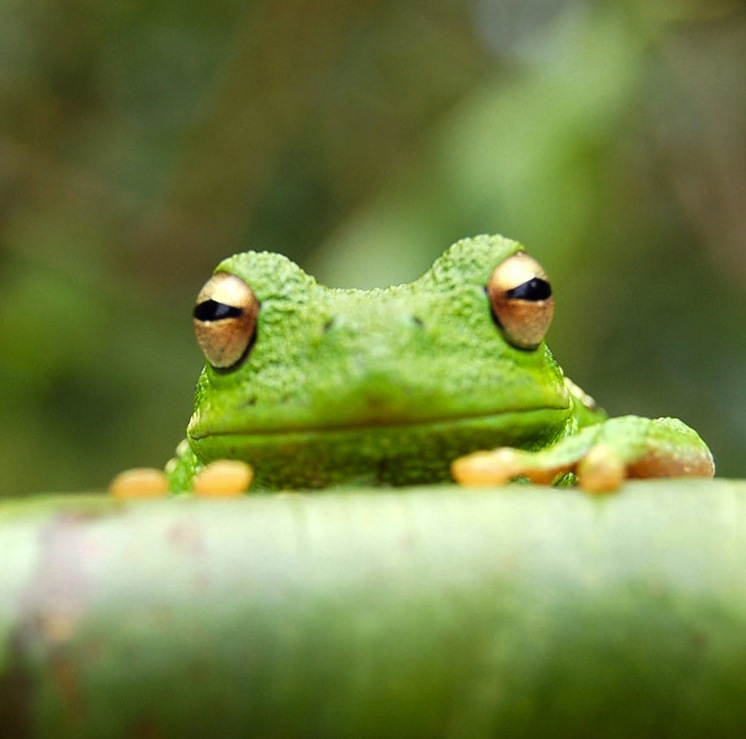
\includegraphics[width=0.25\linewidth]{frog.jpg} 
\caption{\label{fig:frog}This frog was uploaded via the file-tree menu.}
\end{figure}

\subsection{How to add Tables}

Use the table and tabular environments for basic tables --- see Table~\ref{tab:widgets}, for example. For more information, please see this help article on \href{https://www.overleaf.com/learn/latex/tables}{tables}. 

\begin{table}
\centering
\begin{tabular}{l|r}
Item & Quantity \\\hline
Widgets & 42 \\
Gadgets & 13
\end{tabular}
\caption{\label{tab:widgets}An example table.}
\end{table}

\textcolor{Aquamarine}{Tables mostly start in statistical software and end up in \LaTeX. While it is possible to hand-enter results into Overleaf, or export directly in Tex formatting, many people detour through Excel first, either to format the tables first, or to concatenate multiple model's outputs. Sites like \href{https://www.tablesgenerator.com/}{this} will allow you to upload or copy and paste in Excel tables, and will spit out the \LaTeX code needed to create those tables. }


\subsection{How to add Comments and Track Changes}

Comments can be added to your project by highlighting some text and clicking ``Add comment'' in the top right of the editor pane. To view existing comments, click on the Review menu in the toolbar above. To reply to a comment, click on the Reply button in the lower right corner of the comment. You can close the Review pane by clicking its name on the toolbar when you're done reviewing for the time being.

Track changes are available on all our \href{https://www.overleaf.com/user/subscription/plans}{premium plans}, and can be toggled on or off using the option at the top of the Review pane. Track changes allow you to keep track of every change made to the document, along with the person making the change. 

\subsection{How to add Lists}

You can make lists with automatic numbering \dots

\begin{enumerate}
\item Like this,
\item and like this.
\end{enumerate}
\dots or bullet points \dots
\begin{itemize}
\item Like this,
\item and like this.
\end{itemize}

\subsection{How to write Mathematics}

\LaTeX{} is great at typesetting mathematics. Let $X_1, X_2, \ldots, X_n$ be a sequence of independent and identically distributed random variables with $\text{E}[X_i] = \mu$ and $\text{Var}[X_i] = \sigma^2 < \infty$, and let
\[S_n = \frac{X_1 + X_2 + \cdots + X_n}{n}
      = \frac{1}{n}\sum_{i}^{n} X_i\]
denote their mean. Then as $n$ approaches infinity, the random variables $\sqrt{n}(S_n - \mu)$ converge in distribution to a normal $\mathcal{N}(0, \sigma^2)$.

\textcolor{Aquamarine}{\latex uses many characters to denote math formatting. If you want to use these characters in text, put a backslash before them. \$ starts and ends in-text math mode, and \# are used to comment out lines. Using two pairs of \$ will turn everything between them into mathmode. Square brackets wit a backslash before the do the same thing for larger chunks of math (like equations), while commands like begin{equation} can make equations that are stored as objects to be linked to and referenced (like the figure is in the figure section) }

\subsection{How to change the margins and paper size}

Usually the template you're using will have the page margins and paper size set correctly for that use-case. For example, if you're using a journal article template provided by the journal publisher, that template will be formatted according to their requirements. In these cases, it's best not to alter the margins directly.

If however you're using a more general template, such as this one, and would like to alter the margins, a common way to do so is via the geometry package. You can find the geometry package loaded in the preamble at the top of this example file, and if you'd like to learn more about how to adjust the settings, please visit this help article on \href{https://www.overleaf.com/learn/latex/page_size_and_margins}{page size and margins}.

\subsection{How to change the document language and spell check settings}

Overleaf supports many different languages, including multiple different languages within one document. 

To configure the document language, simply edit the option provided to the babel package in the preamble at the top of this example project. To learn more about the different options, please visit this help article on \href{https://www.overleaf.com/learn/latex/International_language_support}{international language support}.

To change the spell check language, simply open the Overleaf menu at the top left of the editor window, scroll down to the spell check setting, and adjust accordingly.

\subsection{How to add Citations and a References List}

You can simply upload a \verb|.bib| file containing your BibTeX entries, created with a tool such as JabRef. You can then cite entries from it, like this: \cite{greenwade93}. Just remember to specify a bibliography style, as well as the filename of the \verb|.bib|. You can find a \href{https://www.overleaf.com/help/97-how-to-include-a-bibliography-using-bibtex}{video tutorial here} to learn more about BibTeX.

\textcolor{Aquamarine}{Zotero will automatically do this for you. If you select which sources you wish to export, right click on them, export and select either BibTex or BibLatex, it will download a .bib file for you. You can then upload that .bib file to overleaf, and cite directly from it. The default citation formatting is a little wonky usually, because it is trying to accommodate a multitude of formatting and citation style options, and sometimes googling how to change the cite command to do the format you need is the quickest way to accomplish what you want to. The online community for overleaf is large and very helpful, and most of your problems have already been asked about by someone else and answered in a forum somewhere. I'm adding a few citations from some random articles I uploaded from Zotero, so you can see how the cite and bibliography commands work.} \cite{prieger_local_2023}
\cite{robb_capital_2014}
If you have an \href{https://www.overleaf.com/user/subscription/plans}{upgraded account}, you can also import your Mendeley or Zotero library directly as a \verb|.bib| file, via the upload menu in the file-tree.

\subsection{Good luck!}

We hope you find Overleaf useful, and do take a look at our \href{https://www.overleaf.com/learn}{help library} for more tutorials and user guides! Please also let us know if you have any feedback using the Contact Us link at the bottom of the Overleaf menu --- or use the contact form at \url{https://www.overleaf.com/contact}.

\bibliographystyle{alpha}
\bibliography{sample}

\end{document}